\documentclass{beamer}
\usepackage[utf8]{inputenc}
\usepackage[portuguese]{babel}
\usepackage{amsmath}
\usepackage{subfigure}
\usepackage{booktabs}
\usepackage{mhchem}             % chemical reactions
\usetheme{metropolis}           % Use metropolis theme

\newtheorem{mydefinition}{Definição}

\newcommand{\foreignword}[1]{\textit{#1}}
\newcommand{\toolname}[1]{\textit{#1}}
\newcommand{\fieldR}{\mathbb{R}}
\newcommand{\powerset}{\mathcal{P}}
\newcommand{\probability}{\mathbb{P}}
\newcommand{\expectation}{\mathbb{E}}
\newcommand{\algname}[1]{\texttt{#1}}
\newcommand{\langname}[1]{\texttt{#1}}
\newcommand{\varname}[1]{\texttt{#1}}
\newcommand{\floor}[1]{\lfloor #1 \rfloor}
\newcommand{\ceil}[1]{\lceil #1 \rceil}
\newcommand{\mathsc}[1]{{\normalfont\textsc{#1}}}
\newcommand{\species}[1]{\textit{#1}}
\newcommand{\gender}[1]{\textit{#1}}

\graphicspath{ {img/} }

\title{Identification of cell signaling pathways based on biochemical 
reaction kinetics repositories}
\date{May 2019}
\author{Gustavo Estrela}
\institute{Instituto de Matemática e Estatística \\ 
           Centro de Toxinas, Resposta-imune e Sinalização Celular (CeTICS) \\
           Laboratório Especial de Ciclo Celular, Instituto Butantan}
\begin{document}
\maketitle
    
%Introduction
%- Cell Signaling Pathways;
%- Modeling it mathematically;
%- With a computational working computational model, we can enlight the
%  structure of a change of behaviour of a cell;
%- Creating a model;
    %- find a set of reactions;
    %- estimate the parameters of this model;
%- Lulu Wu created a method that systematically searches for a model, 
  %modifying it incrementally
    %- we can see the problem as a feature selection problem;
    %- it didn't work out so well...
    %- she was only able to reconstruct models if the starting model was
      %already similar to the correct model
    %- this may have happened because: the database could be more nearly
      %complete; the search algorithm could be more general; her cost 
      %function could not penalize well overcomplex functions.
%- We propose then to create a new methodology that overcomes theses 
  %difficulties using a new cost function, defining a broader search 
  %space and using new search algorithms.
%- Objectives of this work.



\section{Introduction}
\begin{frame}{Cell Signaling}
% Antes de mais nada, vamos entender o que são vias de sinalização 
% celular. 
% A sinalização celular faz parte da comunicação das células de um 
% organismo. Um sinal pode avançar 

%\begin{itemize}
%\item{
Cell signaling allows cells to respond to signals that come from its 
environment changing its behaviour accordingly.
%}
\pause
%\item{

This mechanism is essential for many cell functions, including 
reproduction, growth and death.
%}
\pause
%\item{

Understanding the functioning of cell signaling is important in many 
biological areas.
%}
%\end{itemize}
\end{frame}


\begin{frame}{Cell Signaling}
\begin{figure}
    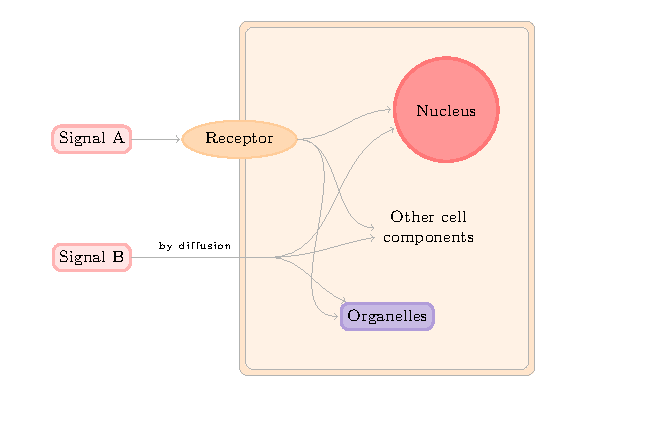
\includegraphics[clip=True, scale=.85]{introduction/signaling_mechanism.pdf}
    \caption{A general cell signaling mechanism.}
\end{figure}
\end{frame}

\begin{frame}{Cell Signaling Pathways}
A cell signaling network can be characterized by a sequence of chemical 
reactions that allows the presence of a signal to modify the state or 
behaviour of a cell.
\begin{figure}
    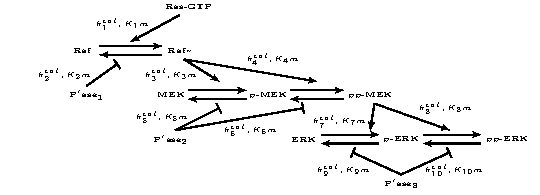
\includegraphics{introduction/csp_example.pdf}
    \caption{An example of a signaling pathway.}
\end{figure}
\end{frame}

\begin{frame}{Mathematical Models of Signaling Networks}
In many applications, we summarize the state of the cell with a 
measurement based on the concentration of chemical species of the cell.
\pause

Using biochemical and enzymatic kinetics, we can write equations that
represent the rate of change of concentration for a chemical species.
\end{frame}


\begin{frame}{Mathematical Models of Signaling Networks}
As an example, for the chemical reaction
\begin{equation*}
\ce{
    A -> B
},
\end{equation*}

\pause
we can write the following equation:
\begin{equation*}
        \frac{d[\text{A}]}{dt} = k_1[\text{A}]; 
\end{equation*}
where $k_1$ is a reaction rate constant.

\pause
Repeating this procedure for all reactions of a pathway allows us to 
derive a system of ordinary differential equations that can model the 
signaling pathway.
% TODO: maybe we should do this more detailed!
\end{frame}


\begin{frame}{Identification of Cell Signaling Pathways}
The problem of identification of cell signaling pathways is the problem
of finding the components of a signaling pathway and how they interact
given a set of experimental measurement.

\pause
As the input, a description of a biological experiment and a set of 
experimental measurements are given. \pause A possible output to the 
problem is composed by:
\begin{itemize}
    \pause
    \item{a model composed by a set of chemical reactions that are 
        relevant for the biological experiment;}
    \pause
    \item{information about the reaction rate constants of the model.}
\end{itemize}
\end{frame}


\begin{frame}{Identification of Cell Signaling Pathways}
One can search for the set of chemical reactions relevant for a 
biological experiment in repositories like the Kyoto Encyclopedia of 
Genes and Genomes (KEGG). \pause However, the pathway maps from KEGG may
be incomplete or have impertinent reactions for the biological 
experiment of interest.
\pause

Hence, it is desirable to construct a method that can systematically 
modify these models and choose the one that better represents the 
experiment.
\end{frame}


\begin{frame}{Identification of Cell Signaling Pathways}
Lulu Wu (2015) presented in her master dissertation a methodology that 
proposes to systematically modify models of signaling network in order
to better represent experiments.
\pause

On her work, the problem of identification of cell signaling pathways is
treated as a feature selection problem.
\end{frame}


\begin{frame}{Feature Selection Problem}
The feature selection problem is a combinatorial optimization problem:
\begin{center}
Given a set of features $S$ and a cost function $c$, find subset 
        $X \in \powerset (S)$, with minimum cost $c(X)$.
\end{center}

\pause
\begin{figure}
    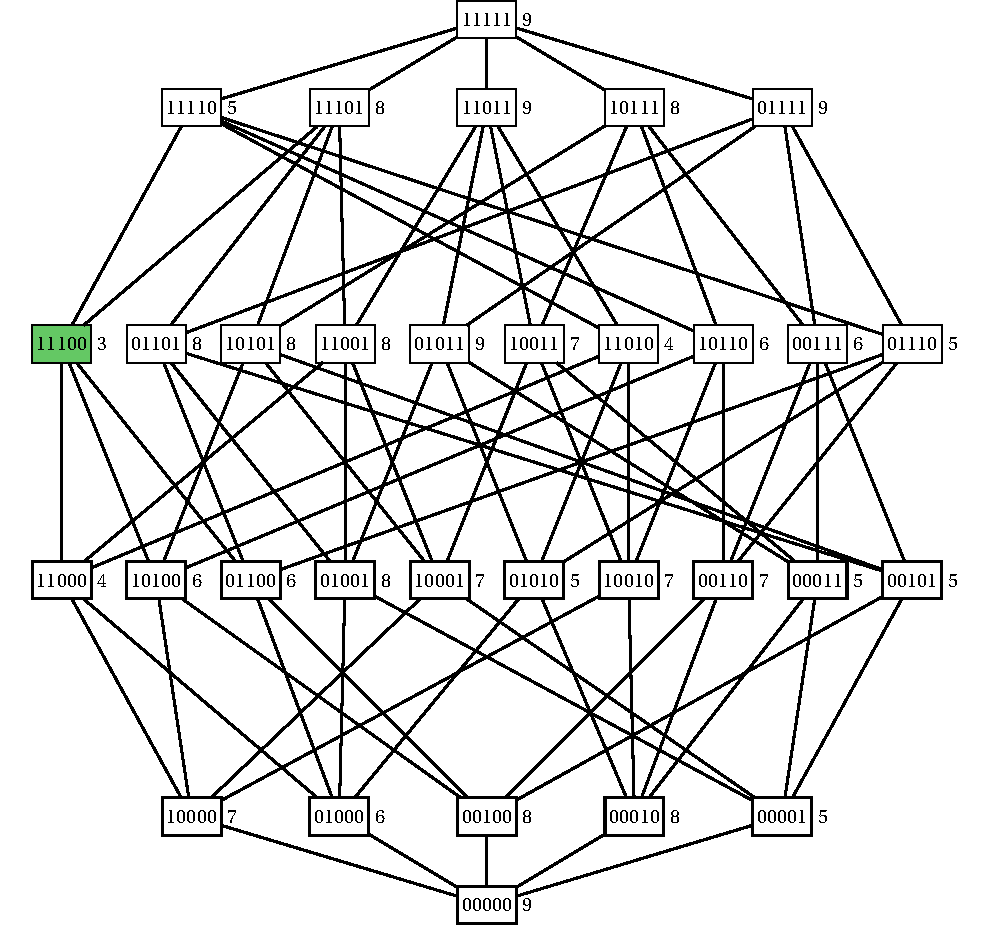
\includegraphics[scale=.24]{introduction/Boolean_lattice.pdf}
    \caption{An example of feature selection search space with 5 
    features.}
\end{figure}
\end{frame}


\begin{frame}{Feature Selection for Identification of Signaling 
Pathways}
The methodology proposed by Wu defines the set of features as a set of 
chemical reactions that can be added to a starting model.\pause This set 
of chemical reactions is fetched from KEGG and stored in a database of
interactions.
\end{frame}


\begin{frame}{Wu's Search Algorithm for Feature Selection}
The search algorithm used by Wu is the Sequential Forward Selection 
(SFS).
\end{frame}


\begin{frame}{Wu's Cost Function for Feature Selection}
Wu defines the cost function as the minimum distance between 
experimental and simulated data. 
\pause
The minimum distance is found using a Simmulated Annealing 
that traverses the parameter space.
\end{frame}


\begin{frame}{Wu's Cost Function for Feature Selection}
If we define that:\pause
\begin{itemize}
    \item{the experimental measurement is $D$;} \pause
    \item{the simulated measure is $\phi (M, \theta)$;} \pause
    \item{all elements visited on the Simmulated Annealing process 
        define $\Theta'$.}
\end{itemize}
\pause
Then, the cost function used on Wu's work is:
\begin{equation*}
    c (M) = min_{\{\theta \in \Theta' \subset \Theta\}}  
        dist (\phi(M, \theta), D) + R (M),
\end{equation*}
\pause
where $R (M)$ is a regularization function.
\end{frame}


\begin{frame}{Wu's Cost Function for Feature Selection}
The $R (M)$ term is implicitly defined by imposing a time limit to the 
Simmulated Annealing procedure used to calculate the cost function. 
\pause As a result, the penalization of the cost function is random.
\end{frame}


\begin{frame}{Results of Wu's Methodology}
Lulu Wu tested her methodology by trying to recreate models given a cut
of the original model. \pause However, the methodology worked 
satisfactorily only when the cut was similar to the original model.
\end{frame}


\begin{frame}{Difficulties of Wu's Methodology}
We can point three aspects of Wu's work that could explain its 
limitation.
\begin{itemize}
\pause
\item{the database of interactions used could be more nearly complete;} 
\pause
\item{the search algorithm could also consider removing interactions;}
\pause
\item{the cost function could implement a proper penalization of 
models;}
\end{itemize}
\end{frame}

% TODO: maybe we should separate this in another section

\begin{frame}{What we Propose on this Project}
We propose to create a methodology that uses a feature selection 
approach for identification of signaling pathways, tackling the 
difficulties encountered by Wu.
\end{frame}


\begin{frame}{What we Propose on this Project}
To get a more nearly complete database of interactions, we should fetch 
information from KEGG and other databases, \pause such as STRING and
SABIO-RK.
\end{frame}


\begin{frame}{What we Propose on this Project}
To create new search algorithms, \pause we intend to use more general
algorithms that can also remove interactions.
\end{frame}


\begin{frame}{What we Propose on this Project}
To define new cost functions, \pause we intend to use Bayesian 
approaches of model selection that allow us to create estimates of 
probabilities such as $p (M | D)$ or $p (D | M)$.
\end{frame}


\begin{frame}{Objectives of this Project}
\begin{itemize}
\pause
\item{Build a database of interactions.}
\pause
\item{Create a cost function for models of signaling pathways.}
\pause
\item{Formulate systematic modifications to a model as the search space
    of a feature selection model.}
\pause
\item{Create search algorithms for the feature selection problem.}
\pause
\item{Test the methodology on known signaling pathways.}
\pause
\item{Apply the methodology on a real case.}
\end{itemize}
\end{frame}


%Fundamental Concepts
%- How are the experimental measures taken
    %- A few details about the procedure
%- How can we model cell signaling pathways mathematically
    %- kinetics laws
    %- M.M. simplifcations
%- How can we choose between models
    %- Approximate Bayesian Computation
    %- Annealing-Melting Integration

% TODO: do we need to talk about western blot?
\section{Fundamental Concepts}


%\begin{frame}{Experimental Measurements of Cell Signaling Pathways}
%Experimental measurements of signaling pathways usually represent the
%ratio of chemical species over time. \pause It is possible to get these
%measurements using a Western blot procedure.
%\begin{figure}
%\end{figure}
%\end{frame}


\begin{frame}{Mathematical Modeling of Enzymatic Reactions}
In this project we use three possible models of kinetics of an 
interaction:
\begin{itemize}
\pause
\item{first order interaction kinetics;}
\pause
\item{second order interaction kinetics;}
\pause
\item{Michaelis-Menten enzymatic kinetics.}
\end{itemize}
\end{frame}


\begin{frame}{Kinetic Model of First Order Iteration}
A first order reaction:
\begin{equation*}
\ce{R ->[\ce{$k_1$}] P},
\end{equation*}
\pause
has rate of:
\begin{equation*}
k_1[R]
\end{equation*}
\end{frame}

\begin{frame}{Kinetic Model of Second Order Iteration}
A first order reaction:
\begin{equation*}
\ce{R_1 + R_2 ->[\ce{$k_1$}] P},
\end{equation*}
\pause
has rate of:
\begin{equation*}
    k_1[R_1][R_2]
\end{equation*}
\end{frame}


%A simple enzymatic equation can be written as:
%\begin{equation*}
%\ce{
    %E + S <=>[\ce{$k$_f}][\ce{$k$_r}] ES ->[\ce{$k_{cat}$}] E + P
%},
%\end{equation*}

%Model Selection
%- Approximate Bayesian Computation
    %- What does it do;
    %- ABC-SMC algorithm
%- A method using Thermodynamic Integration
    %- What does it do;
    %- How to derive the thermodynamic integration
    %- How to estimate this value
% Implementations
\section{Model Selection}


\section{Experiments on Model Selection}
\begin{frame}
\end{frame}
\section{Next Steps}

\end{document}


